\documentclass{beamer}
\usepackage[utf8]{inputenc}

\title{Computação em Nuvem - Aula 3}
\subtitle{Tecnologias de suporte à nuvem\\
Prof. Me. Juliana Costa-Silva}

\usetheme{lucid}

\begin{document}
\frame{
 \titlepage
}

\frame{
    \frametitle{Roteiro de Aula}
    \tableofcontents
}
\section{Arquitetura Orientada a Serviços (SOA)}
\frame {
 \frametitle{Arquitetura Orientada a Serviços (SOA)}
Pensando em sistemas de amplo acesso, um fator relevante foi o desenvolvimento de Arquitetura Orientada a Serviços (SOA – Service Oriented Architectures) (ERL; PUTTINI; MAHMOOD, 2013). Essa arquitetura consiste em decompor as funcionalidades de um sistema em serviços que podem ser reutilizados (CONCEIÇÃO, 2014). O objetivo principal desse estilo arquitetural é promover a interoperabilidade entre aplicações. Neste caso, os serviços devem ser especificados de forma abstrata, sem dependên- cias em relação a plataformas ou linguagens de programação.
 
 \begin{block}{Conceito de Virtualização}
 \begin{itemize}
     \item Os softwares de virtualização permitem a criação de múltiplas instâncias lógicas de um recurso computacional de forma que esse recurso possa ser compartilhado entre diversos usuários. \\
    \item O conceito de virtualização não é recente, mas, somente com os ganhos em termos de desempenho e confiabilidade das ferramentas de virtualização modernas é que foi possível viabilizar características como a elasticidade rápida e self-service sob demanda, próprias dos serviços de computação em nuvem.
    \end{itemize}
 \end{block}
}

\frame {
 \frametitle{Virtualização esquema}
\begin{center}
    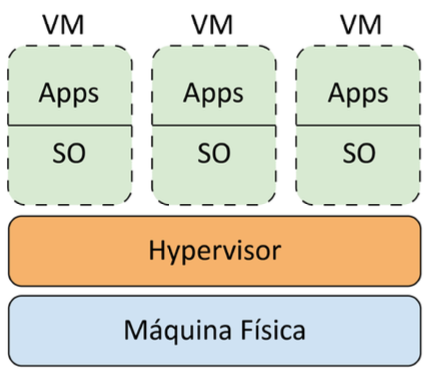
\includegraphics[width=0.4\linewidth]{fig/aula3/aula3_1.png}\\
    \tiny{Fonte: \cite{malheiros2019cc}}
\end{center}
A virtualização pode ser definida como “uma tecnologia que permite criar vários ambientes simulados ou recursos dedicados a partir de um único sistema de hardware físico” \cite{redhat2019}.
} 
\section{Fatores CC}
\frame {
 \frametitle{Fatores da Computação em Nuvem}
 \framesubtitle{Viabilizados pelas VMs}
 A virtualização viabiliza três fatores fundamentais para a computação em nuvem: independência de hardware, possibilidade de consolidação de servidores e facilidade de replicação de recursos \cite{erl2013cloud}.
    \begin{enumerate}
        \item Independência de hardware;
        \item Consolidação de servidores;
        \item Facilidade de replicação.
    \end{enumerate}
} 

\frame{
\frametitle{Independência de hardware}
\begin{block}{Características}
A ferramenta de virtualização abstrai as peculiaridades dos recursos físicos, de forma que problemas de compatibilidade são minimizados. \\
Assim, a migração de uma aplicação em uma máquina virtual não depende das características do hardware do equipamento de destino, desde que o formato da máquina virtual seja suportado pelo hypervisor.
\end{block}
}

\frame{
    \frametitle{Consolidação de servidores}
    \begin{block}{Características}
    A consolidação de servidores é um processo para aumentar a taxa de utilização dos servidores em um centro de dados a fim reduzir custos e economizar energia (AHMAD, 2015). Uma das formas de consolidação de servidores é migrar as máquinas virtuais para o menor número possível de servidores. \\
    \textbf{Por exemplo}, se existe apenas uma máquina virtual em um servidor, ela pode ser migrada para outro servidor que ainda tem recursos disponíveis para que, o primeiro servidor, agora sem nenhuma máquina virtual, possa ser desligado.
    \end{block}
}

\frame{
    \frametitle{Facilidade de replicação}
    \begin{block}{Características}
    O terceiro fator importante é a facilidade na replicação das instâncias de máquinas virtuais. \\
    Isso decorre do fato de que a máquina virtual é software e pode ser replicada com operações simples de manipulação de arquivos. \\
    Assim, é mais fácil instanciar e replicar máquinas virtuais do que servidores físicos.
    \end{block}
}

\frame{
\frametitle{Contêiner de aplicação}
Um modelo alternativo à virtualização baseada em hypervisor é a virtualização baseada em contêiner, que ocorre no nível do sistema operacional \cite{bachiega2017avaliaccao}. 
\begin{center}
    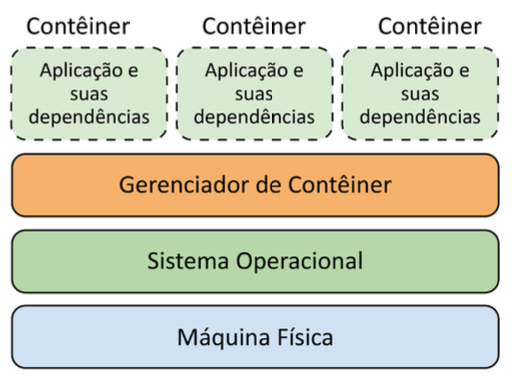
\includegraphics[width=0.6\linewidth]{fig/aula3/aula3_2.png}\\
    \tiny{Fonte: \cite{malheiros2019cc}}
\end{center}
}
\frame{
\frametitle{Contêiner de aplicação}
Neste caso, um conceito importante é o contêiner de aplicação (\textit{Application Container}) que pode ser entendido como um componente de software autossuficiente, no sentido em que ele encapsula uma aplicação e todas as suas dependências (como bibliotecas, arquivos de configuração, etc.) \cite{silva2013abordagem}.

}
\frame{
\frametitle{Fundamentos de computação em nuvem}
\framesubtitle{Vamos jogar!}
\begin{center}
    Acesse Kahoot: www.kahoot.it\\
    Digite o código: na tela.
\end{center}
}

\section{Atividade -Pesquisa}
\frame {
 \frametitle{Atividade de aula}
  Quais são as principais tendências de mercado em Computação em Nuvem (\textit{Cloud Computing}) para 2022?
 
 %https://www.terra.com.br/noticias/tecnologia/conheca-as-tendencias-tecnologicas-em-nuvem-para-2022,4bc56042f4c143ba7b1921c0687ea5c0uouwch32.html
 Leia o artigo Disponível na página da disciplina e responda:

\begin{enumerate}
    \item Qual o objetivo do texto?
    \item Dentre as tendências apresentadas no texto, destaque a que você acredita ser mais promissora e por que?
    \item Na tendência \textbf{Plataforma Cloud-Native}, quais as principais vantagens e desvantagens? Justifique.
    \item Referente aos termos: Computação distribuída, Computação em cluster e computação em grade, quais as diferenças?
    \item Liste as referências utilizadas na pesquisa. Informe no mínimo: Título, Ano e Autor de cada referência.
\end{enumerate}

}

\begin{frame}{Referências}%[allowframebreaks]
 \tiny
 \begin{center}
 	\bibliographystyle{apalike}
	 \bibliography{ref}
 \end{center}
 \end{frame}

\end{document}